\begin{figure}[htbp]
    \centering
    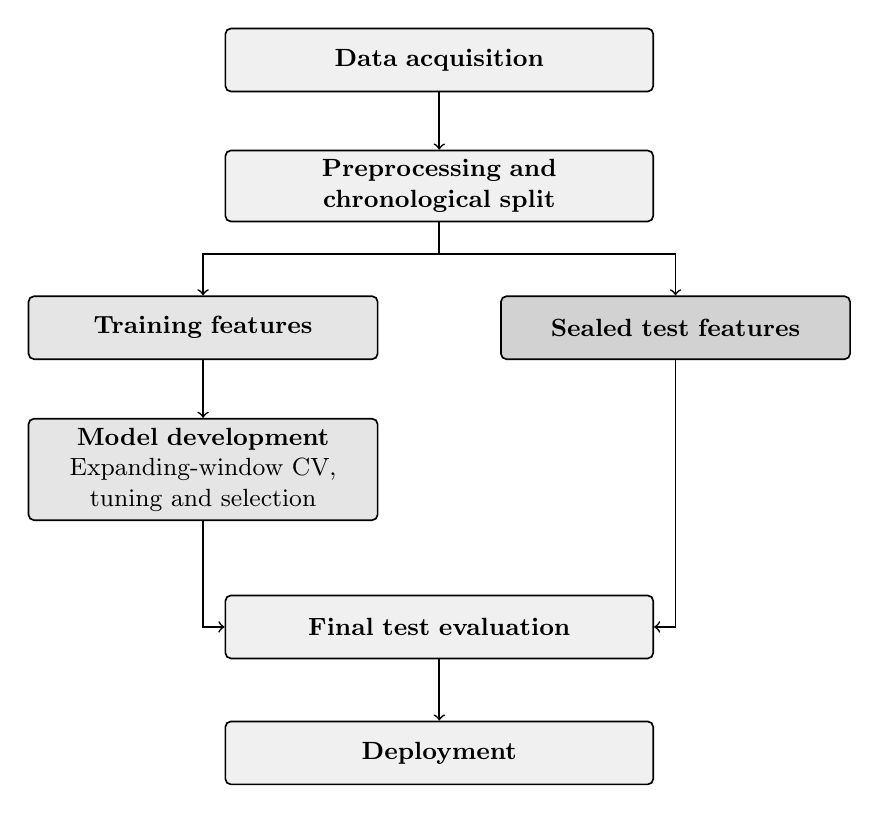
\begin{tikzpicture}[
        font=\small,
        box/.style={
            draw,
            rounded corners=2pt,
            minimum height=0.8cm,
            text width=5.2cm,
            align=center,
            fill=gray!12
        },
        branch/.style={
            draw,
            rounded corners=2pt,
            minimum height=0.8cm,
            text width=4.2cm,
            align=center,
            fill=gray!20
        },
        every path/.style={line width=0.6pt}
    ]

    \node[box] (data) at (0,0)
        {\textbf{Data acquisition}};

    \node[box] (prep) at (0,-1.6)
        {\textbf{Preprocessing and chronological split}};

    \node[branch] (train) at (-3.0,-3.4)
        {\textbf{Training features}};
    \node[branch, fill=gray!35] (test) at (3.0,-3.4)
        {\textbf{Sealed test features}};

    \node[branch] (dev) at (-3.0,-5.2)
        {\textbf{Model development}\\Expanding-window CV, tuning and selection};

    \node[box] (eval) at (0,-7.2)
        {\textbf{Final test evaluation}};

    \node[box] (deploy) at (0,-8.8)
        {\textbf{Deployment}};

    \draw[->] (data) -- (prep);
    \draw[->] (prep.south) -- ++(0,-0.4) -| (train.north);
    \draw[->] (prep.south) -- ++(0,-0.4) -| (test.north);
    \draw[->] (train) -- (dev);
    \draw[->] (dev.south) |- (eval.west);
    \draw[->] (test.south) |- (eval.east);
    \draw[->] (eval) -- (deploy);

    \end{tikzpicture}

    \caption{Overview of the end-to-end pipeline.}
    \label{fig:methodological-pipeline}
\end{figure}
